\documentclass[12pt,a4paper]{ctexart}
\usepackage{amsmath,amssymb,amsfonts}
\usepackage{booktabs}
\usepackage{graphicx}
\usepackage{geometry}
\usepackage{setspace}
\usepackage{titlesec}
\usepackage{enumitem}
\usepackage{array}
\usepackage{longtable}
\usepackage{multirow}
\usepackage{hyperref}
\usepackage[backend=biber,style=numeric,sorting=none]{biblatex}

% 设置上标引用格式
\renewcommand*{\cite}{\supercite}

% 定义新的列类型
\newcolumntype{C}[1]{>{\centering\arraybackslash}p{#1}}
\newcolumntype{L}[1]{>{\raggedright\arraybackslash}p{#1}}

\geometry{left=2cm,right=2cm,top=2cm,bottom=2cm}
\onehalfspacing

% 定义定理环境
\newtheorem{theorem}{定理}[section]
\newtheorem{definition}{定义}[section]

\addbibresource{references.bib}

\begin{document}

% ========== 第一页：开题报告表 ==========
\begin{table}[htbp]
\centering
\renewcommand{\arraystretch}{1.5}
\begin{tabular}{|C{2cm}|C{3.5cm}|C{2cm}|C{5cm}|}
\hline
\multicolumn{4}{|c|}{\textbf{\Large 上海财经大学}} \\ \hline
\multicolumn{4}{|c|}{\textbf{\Large 研究生申请学位论文开题报告表}} \\ \hline
姓名 & 李婧漪 & 学\quad 院 & 统计与数据科学学院 \\ \hline
学号 & 2025213360 & 导师姓名 & 刘旭 \\ \hline
专业 & 应用统计 & 培养层次 & \textbf{专业型硕士} \\ \hline
 &  & \multicolumn{2}{l|}{\textbf{同意开题。}\quad 导师签字：\underline{\hspace{3cm}}} \\ \hline
论文题目 & \multicolumn{3}{l|}{半监督双重稳健Kink回归模型处理效应检验方法研究} \\ \hline
开题时间 & 2026.6.8 & 开题地点 & 统计与数据科学学院208 \\ \hline
\multirow{3}{*}{\parbox{2cm}{\centering 与会专家姓名、单位3-5人}} & & & \\
\cline{2-4}
 & & & \\
\cline{2-4}
 & & & \\ \hline
\multirow{1}{*}{\parbox{2cm}{\centering 开题\\报告\\情况}} & \multicolumn{3}{l|}{\parbox{10.5cm}{专家主要意见：\\[3cm]}} \\ \hline
\multirow{1}{*}{\parbox{2cm}{\centering 开题\\结果\\（划圈）}} & \multicolumn{3}{l|}{\parbox{10.5cm}{
\quad 开题通过，同意进入论文写作阶段。\\[0.5em]
\quad 开题未通过，不同意进入论文写作阶段。\\[1em]
\textbf{开题报告会专家组组长签名：\underline{\hspace{3cm}}}\\[1em]
\textbf{导师签名：\underline{\hspace{3cm}}}\quad 年\quad 月\quad 日
}} \\ \hline
\multicolumn{4}{|l|}{\parbox{12.5cm}{\small 注：填写本表1份，申请开题须经导师签字同意；开题结果由开题报告会专家组组长及导师签署并签字；交研究生秘书进入教学管理信息系统录入开题结果。\\
\textbf{附：上海财经大学研究生学位论文开题报告书（见下页）} 打印3-5份交学院安排开题。}} \\ \hline
\end{tabular}
\end{table}

\newpage

% ========== 第二页：开题报告书封面 ==========
\begin{center}
\vspace{2cm}
{\LARGE \textbf{上海财经大学}}\\[1em]
{\LARGE \textbf{研究生学位论文开题报告书}}\\[3em]
{\Large \textbf{论文题目：半监督双重稳健Kink回归模型处理效应检验方法研究}}\\[4em]
\end{center}

\begin{center}
\large
\begin{tabular}{rl}
\textbf{姓\quad 名：} & 李婧漪 \\[0.8em]
\textbf{学\quad 号：} & 2025213360 \\[0.8em]
\textbf{院系所：} & 统计与数据科学学院 \\[0.8em]
\textbf{专\quad 业：} & 应用统计 \\[0.8em]
\textbf{培养层次：} & 专业型硕士 \\[0.8em]
\end{tabular}
\end{center}

\newpage

\section{选题的背景、研究问题、理论意义、实用价值}

\subsection{选题背景}

在医疗检验与因果推断领域，处理效应的异质性检验是一个核心问题。传统的因果推断方法通常假设处理效应在所有个体中是同质的，但在实际经济与社会科学场景中，处理效应往往随某个连续变量（如收入、年龄、教育年限等）的变化而发生结构性改变，即存在所谓的"拐点"（Kink）效应。例如，税收政策对劳动供给的影响可能在某个收入阈值处发生斜率变化；医保补贴对医疗支出的影响可能在某个年龄节点处出现结构性转折。

图\ref{fig:kink_illustration}直观展示了Kink回归模型的核心特征。图\ref{fig:kink_illustration}(a)显示，回归函数在拐点$\delta$处连续但斜率发生突变：在$\delta$左侧，回归函数斜率为$\alpha_1$；在$\delta$右侧，斜率变为$\alpha_1 + \tau$。参数$\tau$即为Kink效应的大小，表示斜率在拐点处的变化量。图\ref{fig:kink_illustration}(b)进一步展示了处理效应的Kink型异质性：在拐点之前，处理组与对照组的响应曲线平行（处理效应为零）；在拐点之后，两组曲线逐渐分离，处理效应随运行变量$X$的增大而增强。这种设定在医学研究中尤为常见——例如，某种药物可能仅在患者年龄超过某个阈值后才显著改善预后，且改善程度随年龄继续增加。

\begin{figure}[htbp]
\centering
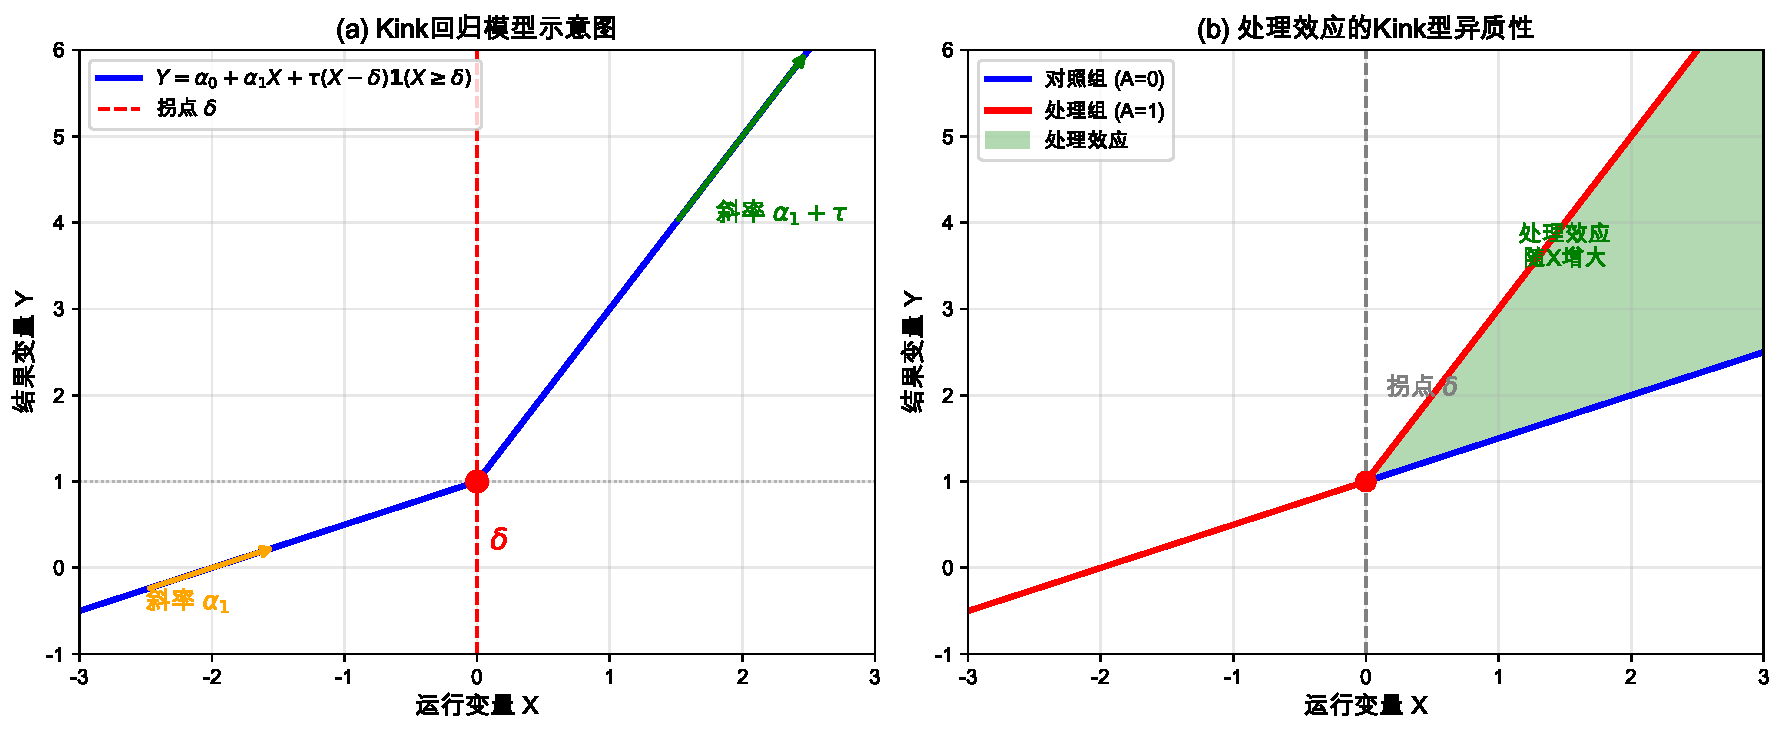
\includegraphics[width=0.95\textwidth]{kink_illustration.pdf}
\caption{Kink回归模型示意图}
\label{fig:kink_illustration}
\small
\textbf{注}：(a) Kink回归函数在拐点$\delta$处连续但斜率发生突变；(b) 处理效应的Kink型异质性，处理效应仅在拐点之后显现并随运行变量增大而增强。
\end{figure}

与此同时，大数据时代的实证研究普遍面临"标签稀缺"问题：虽然协变量和处理分配信息容易大规模获取，但结果变量的收集往往成本高昂（如需要长期追踪调查、实验测量等）。这种半监督（Semi-supervised）数据结构——少量有标签数据（Labeled data）与大量无标签数据（Unlabeled data）并存——在医学研究、社会调查、经济统计中极为常见。如何充分利用无标签数据中的协变量信息来提升检验的统计效率，是一个兼具理论深度和实际紧迫性的研究问题。

\subsection{研究问题}

本文聚焦以下核心问题：

（1）如何在Kink回归模型中构建半监督双重稳健（Doubly Robust）检验统计量，使得当倾向分数模型或基线结果模型中至少一个正确设定时，检验在零假设下仍具有正确的Type I Error控制；

（2）如何通过非参数插补（Imputation）策略将无标签数据的信息融入检验过程，实现渐近方差的严格缩减，从而提升检验功效；

（3）如何设计计算高效的乘数自助法（Multiplier Bootstrap）来逼近检验统计量的极限零分布，避免传统自助法在大规模无标签数据下的计算瓶颈。

\subsection{理论意义}

第一，本文将双重稳健推断从全监督框架推广至半监督框架，证明在零假设下检验统计量依分布收敛于一个零均值高斯过程的上确界（定理1），且该收敛在倾向分数模型或基线结果模型任一正确设定时均成立，为半监督因果推断提供了新的理论保障。

第二，本文严格证明了半监督score函数的渐近方差满足$\Sigma_{SS}(\delta) = \Sigma_1(\delta) - \Delta(\delta)$，其中$\Delta(\delta) \geq 0$，且在$\mathrm{Var}(E[\psi_1|X,W,A]) > 0$时$\Delta(\delta) > 0$严格成立（定理2）。这从理论上确认了半监督方法的效率增益。

第三，在局部替代假设$H_{1n}: \tau = n^{-1/2}c_0$下，本文推导出检验统计量的非中心参数$\mu_{SS}(\delta)$严格大于全监督的对应量（定理3），从漂移函数的角度解释了方差缩减如何转化为功效提升。

第四，本文提出基于adjusted influence function的乘数自助法，并证明其条件分布一致性（定理4），为实际中临界值的计算提供了理论依据。

\subsection{实用价值}

本研究的实用价值体现在以下几个方面：

（1）医疗研究中的异质性效应检验。在评估药物治疗、临床干预或肿瘤风险因素的作用效果时，研究者常需判断治疗效应是否会随着年龄、生物指标等运行变量（Running Variable）的变化而发生结构性改变。本文方法能够同时估计拐点位置并检验处理效应的存在性，从而识别不同患者群体中的关键风险阶段，为精准医疗和个体化预后评估提供统计依据。

（2）半监督数据的高效利用。在实际调查中，协变量和处理分配信息通常可以大规模获取（如行政记录、注册数据），而结果变量（如健康状况、收入变化）仅在小样本中被观测。本文方法通过非参数插补充分利用无标签数据，在不增加标签成本的前提下提升检验功效。

（3）双重稳健性保障。在因果推断中，倾向分数模型和结果模型往往难以同时正确设定。本文方法只需其中一个正确即可保证Type I Error控制，降低了模型误设的风险，增强了实际应用的稳健性。

（4）计算可行性。乘数自助法仅需一次估计倾向分数和基线模型，避免了传统自助法中反复重新估计的巨大计算开销，使得在大规模无标签数据下的推断变得可行。

\section{国内外研究现状与发展趋势}

\subsection{Kink回归与结构性变化检验}

结构性变化的检测是统计学的经典问题。\cite{chow1960}提出了已知断点下的结构性变化检验，奠定了该领域的理论基础。此后，研究者逐步将注意力转向未知断点情形：\cite{andrews1993}发展了未知变化点的sup-Wald检验，证明了极限分布为样本路径上确界的布朗运动泛函；\cite{hansen1996}进一步研究了nuisance参数在零假设下不被识别时的推断问题，提出了固定回归的自助法（Fixed regressor bootstrap）来逼近极限分布。

门槛回归（Threshold regression）模型允许回归函数在断点处不连续跳变，\cite{hansen2000}系统发展了门槛回归的估计与推断理论，提出了基于最小二乘的门槛估计量和基于自助法的推断方法，成为该领域的标志性工作。然而，在许多实际应用中，回归函数在变化点处是连续的但斜率发生变化——即"拐点"（Kink）情形——这一约束比门槛模型更为合理，尤其在医学、生物统计当中更具有实际应用价值。\cite{calonico2014}发展了RKD中局部多项式估计的稳健偏倚校正推断方法，此后\cite{card2017}进一步研究了Kink点的估计与推断问题。

近年来，Kink回归的研究呈现出两个重要趋势。第一，从参数化模型向半参数化、非参数化方向拓展。\cite{wang2025}提出了尖锐回归拐点设计中局部处理效应的统一识别与推断框架，将方法推广至均值、分位数和不平等测度等Hadamard可微泛函，使用局部多项式约束回归进行估计并建立了渐近理论和有效的重抽样程序。\cite{ghosh2025}研究了动态门槛设计中的非参数因果推断，考虑了处理分配由状态变量门槛化决定的时序设定，证明了动态门槛设计可识别边际政策效应，并提出了定制的局部线性回归估计量，应用于连续血糖监测的阈值优化问题。

第二，从单纯的拐点估计向处理效应异质性检验深化。\cite{calonico2025}发展了回归断点设计中处理效应异质性分析的统一框架，使用完全交互的局部线性模型，建立了带宽选择准则和稳健偏倚校正推断方法，为异质性处理效应的组间差异检验提供了理论依据。然而，上述工作均基于全监督框架，未考虑无标签数据的利用，这恰好是本文的研究切入点。

\subsection{双重稳健推断方法}

双重稳健（Doubly Robust, DR）估计由\cite{robins1994}提出，其核心优势在于倾向分数模型或结果回归模型中至少一个正确设定时，估计量仍具有一致性。这一性质使得双重稳健方法在模型误设风险较高的实际应用中具有重要价值。\cite{bang2005}进一步将双重稳健方法拓展至边际结构模型的估计，\cite{vanderlaan2011}在目标学习（Targeted Learning）框架下系统发展了双重稳健估计理论。

近年来，双重稳健方法的研究在以下方向取得了重要进展。第一，双重稳健估计的最优性理论。\cite{jin2024}在结构不可知（Structure-agnostic）框架下，证明了双重稳健估计在处理效应估计中的统计最优性：仅假设对nuisance函数有黑箱估计器达到某个统计估计率，双重稳健估计即可达到ATE和ATT的最小最大最优率。该工作从理论上确认了双重稳健方法在处理效应估计中的根本地位。\cite{jin2025}进一步建立了更一般的线性泛函估计的最优下界，刻画了何时可以实现双重稳健性、何时不可实现的精确条件。

第二，双重稳健检验方法的拓展。\cite{jain2026}提出了条件分布处理效应的双重稳健估计与检验方法，关注处理如何影响整个结果分布（而非仅均值），发展了最小最大最优双重稳健估计量，并构建了条件潜在结果分布全局齐一性的检验——这是首个同时保证Type I Error有效性和对固定替代一致性的检验。\cite{boileau2025}提出了基于方差的异质性处理效应检测方法，当效应修饰变量被遗漏或误测量时，传统的CATE方法失效，该文通过潜在结果方差的对比来检验齐一处理效应假设，发展了双重稳健的、渐近线性的因果机器学习估计量。

第三，双重稳健方法在非参数和因果推断前沿的应用。\cite{ghassami2025}提出了去偏不适定回归方法，将双重稳健策略应用于非参数工具变量估计和近端因果推断；\cite{hui2025}提出了基于深度学习的双重稳健Granger因果检验，使用神经网络处理高维滞后阶数，通过乘数自助法获取临界值，证明了检验的Type I Error渐近有效性和功效一致性。这些工作表明，双重稳健方法正从传统的参数/半参数估计拓展至更广泛的检验与推断场景，本文将双重稳健构造首次引入半监督Kink检验，正是这一趋势的延伸。

\subsection{半监督统计推断}

半监督统计推断是近年来因果推断与统计学交叉领域的研究热点。其核心思想是：在标签稀缺但协变量丰富的场景下，利用无标签数据中的协变量分布信息来提升估计或推断的精度。\cite{zhang2022}发表了半监督框架下均值推断的开创性工作，证明了利用无标签数据可以实现比全监督方法更短的置信区间，首次在半监督设定下建立了效率增益的严格理论。

\cite{chakrabortty2024}提出了半监督和高维设定下处理效应估计的一般框架，同时考虑了平均处理效应（ATE）和分位数处理效应（QTE），证明当倾向分数正确设定时，半监督估计量比全监督对应量更稳健且更高效，在所有nuisance函数正确设定时可达半参数有效界。该工作还建立了高维设定下核平滑估计量的一致收敛速率，为半监督因果推断的高维推广提供了技术工具。

\cite{zhang2023}提出了衰减缺失随机（Decaying MAR）框架下的模型双重稳健因果推断方法。该框架处理了半监督设定中标签概率随协变量衰减的重要情形，提出了偏差缩减半监督（BRSS）估计量和去耦BRSS（DC-BRSS）估计量，进一步放松了模型设定和稀疏性要求，实现了在衰减标签概率下的渐近正态性。

\cite{kato2025}研究了半监督设定中利用未标记辅助协变量的处理效应估计，建立了效率界并发展了达到效率界的估计量，证明了引入辅助协变量可以降低效率界，为半监督因果推断中协变量选择提供了理论指导。

在效率增益的理论刻画方面，现有半监督因果推断文献主要关注点估计的效率提升，而对检验问题中方差缩减如何转化为功效提升的机理缺乏严格分析。本文在Kink回归模型的半监督双重稳健检验中，严格证明了渐近方差满足$\Sigma_{SS}(\delta) = \Sigma_1(\delta) - \Delta(\delta)$且$\Delta(\delta) > 0$，并在局部替代假设下推导出非中心参数的严格放大，从漂移函数的角度解释了方差缩减到功效提升的转化机制，填补了半监督检验理论中的这一空白。

\subsection{非参数核估计与乘数自助法}

单指标模型（Single-index model）是非参数统计的重要工具，通过将高维协变量投影到一维指标上来克服"维数灾难"。Nadaraya-Watson（NW）核估计是该领域的经典方法。\cite{ichimura1993}提出了单指标模型的半参数最小二乘估计，\cite{hardle1993}发展了单指标模型的NW核估计理论。本文采用单指标NW核估计来非参数地估计$m(X,W) = E[Y|h(X,W;\hat{\zeta})]$，以$h$的线性预测值作为单指标，有效规避了高维核估计的维数灾难问题。

在单指标模型的推断方面，\cite{tang2024}建立了部分线性单指标模型中平滑样条估计量的Bahadur表示，证明了连接函数估计量与指标系数估计量的联合弱收敛和渐近独立性，发展了同时置信带和乘数自助法程序。这一工作为单指标模型的同时推断提供了理论工具，与本文中NW核估计的理论性质密切相关。

乘数自助法（Multiplier bootstrap）由\cite{mammen1993}引入，其核心思想是通过乘数扰动（而非重抽样）来模拟估计量的极限分布。相较于传统非参数自助法，乘数自助法仅需一次估计nuisance参数，通过高斯扰动生成扰动统计量，计算效率极高，特别适合$N$远大于$n$的半监督场景。

近年来，乘数自助法在多个方向得到拓展和应用。\cite{shang2025}提出了数据整合下非参数推断的乘数自助法程序，在协变量偏移和分布偏移两种场景下建立了自助法一致性，为目标均值函数的局部和全局推断提供了计算便捷的推断方法。\cite{song2026}发展了基于投影的非参数显著性检验和条件独立性检验，使用定制的投影加权函数使检验能以参数速率检测局部替代，并采用乘数自助法获取临界值，克服了现有方法对协变量密度紧支撑的较强假设。

在sup-type检验统计量的推断方面，乘数自助法的有效性需要特别关注。由于检验统计量为高斯过程样本路径的上确界，其极限分布依赖于未知的数据生成机制，解析推导临界值不可行。本文提出基于adjusted influence function的乘数自助法，将nuisance参数的一阶估计误差从score函数中投影出去，保证了扰动统计量的条件分布一致性，为半监督sup-type检验统计量的临界值计算提供了理论上可靠且计算上高效的方法。

\subsection{文献述评}

综合以上四个方面的文献梳理，现有研究存在以下不足：

第一，Kink回归的检验方法主要基于全监督框架，未考虑无标签数据的利用。虽然\cite{calonico2014}、\cite{wang2025}等在Kink点的估计与推断方面取得了重要进展，但均假设所有观测的结果变量均可获得。在标签稀缺的实际场景下，这些方法的检验功效受到标记样本量的限制，无法充分利用大规模无标签数据中的协变量信息。

第二，半监督因果推断的研究主要聚焦于点估计（ATE、QTE等），对检验问题的关注不足。\cite{chakrabortty2024}、\cite{zhang2023}等虽然在半监督处理效应估计方面取得了重要突破，但主要讨论估计的效率和稳健性，尚未系统研究半监督框架下结构性变化检验的统计性质。特别是方差缩减如何转化为检验功效提升的机理，在现有文献中缺乏严格的理论刻画。

第三，现有的双重稳健检验方法（如\cite{jain2026}、\cite{boileau2025}）虽然将双重稳健构造推广到了更丰富的检验场景，但均未在半监督框架下进行。半监督设定下的双重稳健检验需要同时处理合并倾向分数估计、非参数插补和adjusted influence function，其渐近性质与全监督情形有本质区别，需要专门的理论分析。

本文的研究定位正是填补上述空白：在Kink回归模型中，首次构建半监督双重稳健检验统计量，利用合并倾向分数估计和非参数score插补将无标签数据的信息融入检验过程；严格证明渐近方差的缩减和功效的提升；提出基于adjusted influence function的乘数自助法来高效逼近极限零分布。本文的研究位于Kink回归、双重稳健推断和半监督统计推断三个领域的交叉点，在理论方法上具有明确的创新性和前沿性。

\section{研究的基本思路与方法}

本文研究在Kink回归模型中如何构建半监督双重稳健（Doubly Robust）检验统计量，在传统全监督双重稳健score检验的基础上，引入半监督数据结构，通过合并估计倾向分数、非参数插补未标记样本score、adjusted influence function校正和乘数自助法推断，构造在模型误设下仍具有稳健性、并能利用无标签数据提高检验效率的统计方法。具体而言，本文并不直接估计某一个固定拐点处的处理效应，而是在未知拐点$\delta$的搜索空间内构造一族标准化score过程，通过其上确界统计量判断是否存在处理效应斜率的结构性变化。

\subsection{模型设定}

考虑如下半监督Kink回归模型：
\begin{equation}
Y = \alpha_0 + \alpha_1 X + \tau A(X - \delta)\mathbf{1}(X \geq \delta) + \mu(W) + \varepsilon
\label{eq:model}
\end{equation}
其中$Y$为结果变量，$X$为运行变量，$A\in\{0,1\}$为处理指示变量，$W$为$p$维协变量，$\delta$为未知的拐点，$\tau$为拐点处处理效应的斜率变化，$\mu(W)$为协变量的光滑效应函数，$\varepsilon$满足$E[\varepsilon|A,X,W] = 0$。

在半监督设定下，观测数据由标记数据集$\mathcal{L} = \{Z_i = (X_i, W_i, A_i, Y_i): i=1,\ldots,n\}$和未标记数据集$\mathcal{U} = \{(X_j, W_j, A_j): j=n+1,\ldots,n+N\}$组成，其中未标记数据缺失结果变量$Y$，且$N \gg n$。研究目标为检验：
\begin{equation}
H_0: \tau = 0 \quad \text{vs} \quad H_1: \tau \neq 0
\label{eq:hypothesis}
\end{equation}
在$H_0$下，处理效应不存在Kink型异质性，即处理效应不随$X$在某个未知点之后发生斜率突变；在$H_1$下，存在某个$\delta$使得处理组的条件均值函数在该点之后出现斜率变化。由于$\delta$在$H_0$下不可识别，本文不能采用普通Wald检验或单点score检验，而需要在$\delta$的候选集合$\mathcal{D}$上构造sup-type统计量。

数据结构采用半监督设定。标记样本为$\mathcal{L}=\{Z_i=(X_i,W_i,A_i,Y_i): i=1,\ldots,n\}$，同时观测$X$、$W$、$A$和$Y$；未标记样本为$\mathcal{U}=\{(X_j,W_j,A_j): j=n+1,\ldots,n+N\}$，仅观测$X$、$W$和$A$，缺失结果变量$Y$。假定$\mathcal{L}$和$\mathcal{U}$来自同一总体分布，且$N$通常远大于$n$。该设定对应许多实际应用场景：协变量和处理状态可由行政记录或平台数据大规模获得，但结果变量需要调查、追踪或人工标注，成本较高。本文方法的目标是在不额外增加$Y$观测成本的情况下，利用$\mathcal{U}$中丰富的$(X,W,A)$分布信息提高检验效率。

\subsection{半监督双重稳健Score检验}

检验的核心是构建双重稳健的score函数。对于标记数据，score函数为：
\begin{equation}
\psi_1(Z_i; \delta) = (X_i - \delta)\mathbf{1}(X_i \geq \delta) \cdot \{A_i - \hat{\pi}(X_i, W_i)\} \cdot \{Y_i - \hat{h}(X_i, W_i)\}
\label{eq:score_labeled}
\end{equation}
其中$\hat{\pi}$为倾向分数的合并估计（在$\mathcal{L}\cup\mathcal{U}$上拟合），$\hat{h}$为基线结果模型估计。该score函数具有双重稳健性：当$\pi$或$h$中至少一个正确设定时，$E[\psi_1|H_0] = 0$。

对于未标记数据，由于$Y$缺失，用NW核估计$\hat{m}(X,W) = E[Y|h(X,W;\hat{\zeta})]$替换$Y$，得到插补score函数：
\begin{equation}
\bar{\psi}_1(O_j; \delta) = (X_j - \delta)\mathbf{1}(X_j \geq \delta) \cdot \{A_j - \hat{\pi}(X_j, W_j)\} \cdot \{\hat{m}(X_j, W_j) - \hat{h}(X_j, W_j)\}
\label{eq:score_unlabeled}
\end{equation}

半监督score函数为两者的加权平均：
\begin{equation}
\Psi_{SS}(\delta) = \lambda \cdot \frac{1}{n}\sum_{i=1}^{n}\psi_1(Z_i;\delta) + (1-\lambda) \cdot \frac{1}{N}\sum_{j=n+1}^{n+N}\bar{\psi}_1(O_j;\delta)
\label{eq:score_ss}
\end{equation}
其中$\lambda = n/M$，使得每个观测获得等权。

\subsection{检验统计量与推断}

构建sup-type检验统计量：
\begin{equation}
T_{n,SS} = \sup_{\delta \in \mathcal{D}} \left[\frac{\sqrt{n}\cdot\Psi_{SS}(\delta)}{\hat{\sigma}_{SS}(\delta)}\right]^2
\label{eq:test_stat}
\end{equation}
该统计量的含义是：在所有可能拐点中，寻找标准化Kink信号最强的位置。如果$H_0$成立，则整个score过程应围绕0波动；若存在某个真实拐点$\delta_0$，则在$\delta$接近$\delta_0$的位置，score会出现系统性偏离，sup统计量倾向于变大。其中搜索空间$\mathcal{D}$由合并数据$\{X_k\}_{k=1}^M$的次序统计量构造：
\begin{equation}
\mathcal{D} = \left\{\delta_{(k)} : k = \lceil M\theta \rceil, \ldots, \lfloor M(1-\theta) \rfloor\right\}
\label{eq:search_space}
\end{equation}

方差估计$\hat{\sigma}^2_{SS}(\delta)$使用adjusted influence function的样本方差计算。在实际计算中，score不仅包含原始观测误差，还包含$\hat{\eta}$、$\hat{\zeta}$和$\hat{m}$等nuisance参数估计误差。如果直接用原score样本方差估计$\sigma^2_{SS}(\delta)$，可能忽略一阶估计误差对统计量分布的影响，导致临界值和$p$值不准确。因此，本文采用adjusted influence function对score进行校正。

Adjusted influence function通过将nuisance参数的一阶估计误差从score中投影出去获得：
\begin{equation}
\psi^*_{SS} = \psi_{SS} - G\cdot(G'G)^{-1}G'\psi_{SS}
\label{eq:adjusted_if}
\end{equation}
其中$G = [D_\eta\cdot(A-\hat{\pi}), D_\zeta\cdot(Y-\hat{h})]$（标记数据）或$G = [D_\eta\cdot(A-\hat{\pi}), D_\zeta\cdot(\hat{m}-\hat{h})]$（未标记数据）。

\subsection{乘数自助法}

临界值通过乘数自助法获得。生成标准正态随机变量$\xi = (\xi_1,\ldots,\xi_M)$，构造扰动统计量：
\begin{equation}
T^*_{n,SS} = \sup_{\delta \in \mathcal{D}} \frac{1}{\hat{\sigma}^2_{SS}(\delta)} \cdot \left[\sqrt{n} \cdot \left(\frac{\lambda}{n}\sum_{i=1}^{n}\xi_i\psi^*_{SS}(Z_i;\delta) + \frac{1-\lambda}{N}\sum_{j=n+1}^{n+N}\xi_j\psi^*_{SS}(O_j;\delta)\right)\right]^2
\label{eq:bootstrap}
\end{equation}
重复$B$次得到$\{T^{*(b)}\}_{b=1}^B$，其经验分布逼近$T_{n,SS}$在零假设下的极限分布。$p$值为$p = \frac{1}{B}\sum_{b=1}^{B}\mathbf{1}(T^{*(b)} > T_{n,SS})$。

\subsection{模拟实验设计}

为验证理论方法的有限样本表现，设计如下蒙特卡洛模拟实验：

（1）数据生成过程（DGP）：$X \sim \mathrm{Uniform}(-2, 2)$，$W \sim N(0, I_2)$，倾向分数$\pi = \mathrm{logistic}(0.2 + 0.3X - 0.2W_1 + 0.1W_2)$，$Y = 1 + 0.5X + \tau A(X-\delta)\mathbf{1}(X\geq\delta) + 0.3W_1 + 0.2W_2 + \varepsilon$，$\varepsilon \sim N(0,1)$。

（2）参数设置：标记样本量$n \in \{200, 400, 800\}$，未标记/标记比$N/n = 5$，拐点$\delta = 0$，处理效应$\tau \in \{0, 0.3, 0.5, 0.8\}$，显著性水平$\alpha = 0.05$，Bootstrap重复次数$B = 500$，蒙特卡洛重复200次。

（3）评价指标：$\tau = 0$时的Type I Error（应接近$\alpha = 0.05$），$\tau > 0$时的检验功效（拒绝率），以及半监督与全监督方法的功效差异。

\section{论文的创新性尝试}

本文的创新性主要体现在以下两个方面：

\subsection{半监督双重稳健Kink检验的理论框架}

现有Kink回归文献主要在全监督框架下进行检验，无法利用无标签数据中的协变量信息。本文首次在Kink回归模型中构建了半监督双重稳健检验统计量：通过合并估计倾向分数、非参数插补未标记数据的score、以及adjusted influence function校正nuisance参数估计误差，构造了在倾向分数模型或基线结果模型任一正确设定时均能保证Type I Error有效性的检验方法，并发展了计算高效的乘数自助法用于临界值推断。

\subsection{半监督效率增益的严格理论证明}

现有半监督因果推断文献主要关注点估计的效率提升，对检验问题中方差缩减如何转化为功效提升的机理缺乏严格分析。本文证明了半监督score函数的渐近方差满足$\Sigma_{SS}(\delta) = \Sigma_1(\delta) - \Delta(\delta)$且$\Delta(\delta) > 0$严格成立，并在局部替代假设下推导出非中心参数的严格放大，从漂移函数角度解释了方差缩减到功效提升的转化机制，填补了半监督检验理论中的这一空白。

\section{研究难点与预期成果}

\subsection{理论层面}

完成半监督双重稳健Kink检验的完整渐近理论推导，包括定理1（零假设下的极限分布）、定理2（效率增益）、定理3（局部替代下的功效分析）和定理4（乘数自助法一致性）的证明。

\subsection{模拟实验}

\subsubsection{实验设置}

为系统评估所提出方法在不同数据环境下的有限样本表现，本文采用Monte Carlo模拟设计。协变量$X$分别设定为服从均匀分布$X\sim\mathrm{Uniform}(-1,1)$与正态分布$X\sim N(0,1)$，以比较不同协变量分布下方法的稳定性与鲁棒性。有标签样本量$n$分别取200和400，无标签样本量与有标签样本量之比固定为$N/n=5$，以模拟半监督学习中"少量有标签数据与大量无标签数据"并存的典型场景。误差项标准差$\sigma$分别设置为0.5和1.0，用于考察不同噪声水平下方法的表现，并在Type I error结果中同时报告两种噪声情形。kink位置参数$\delta$分别取协变量分布的0.35、0.50与0.65分位点，以对应拐点位于左侧、中部及右侧的不同情形，从而检验方法对拐点位置变化的敏感性。备择强度参数$\tau$分别取0、0.3、0.5与0.8，其中$\tau=0$表示原假设成立，用于评估检验的Type I error，而$\tau>0$用于考察不同信号强度下的检验功效。

模拟中进一步比较三种方法：仅利用有标签样本进行估计与检验的Labeled-only方法、同时结合有标签与无标签样本并基于半监督双重稳健思想构建的Semi-supervised方法，以及假设全部$n+N$个样本响应变量均可观测的Oracle full-data方法作为理想全监督基准。在每次Monte Carlo重复实验中，首先依据给定的数据生成机制生成有标签与无标签样本，再分别计算三种方法对应的检验统计量，并采用Bootstrap方法进行重抽样，Bootstrap次数设定为$B=200$，基于经验分布构造临界值或计算$p$值。显著性水平设定为$\alpha=0.05$，因此在$\tau=0$时拒绝原假设的比例用于衡量Type I error，其理论值应接近0.05；而在$\tau>0$时，拒绝原假设的比例则定义为检验功效（Power）。

\subsubsection{Type I error结果}

\begin{table}[htbp]
\centering
\caption{$X \sim \mathrm{Uniform}(-1, 1)$时的Type I error}
\label{tab:type1_uniform}
\small
\begin{tabular}{ccccccc}
\toprule
delta\_quantile & Method & $\sigma=0.5, n=200$ & $\sigma=0.5, n=400$ & $\sigma=1.0, n=200$ & $\sigma=1.0, n=400$ \\
\midrule
0.35 & Labeled-only & 0.080 & 0.060 & 0.050 & 0.040 \\
0.35 & Semi-supervised & 0.070 & 0.080 & 0.070 & 0.060 \\
0.35 & Oracle full-data & 0.130 & 0.070 & 0.070 & 0.050 \\
\midrule
0.50 & Labeled-only & 0.060 & 0.090 & 0.090 & 0.060 \\
0.50 & Semi-supervised & 0.030 & 0.090 & 0.070 & 0.060 \\
0.50 & Oracle full-data & 0.090 & 0.040 & 0.090 & 0.040 \\
\midrule
0.65 & Labeled-only & 0.030 & 0.020 & 0.060 & 0.010 \\
0.65 & Semi-supervised & 0.040 & 0.050 & 0.060 & 0.030 \\
0.65 & Oracle full-data & 0.100 & 0.060 & 0.060 & 0.090 \\
\bottomrule
\end{tabular}
\end{table}

\begin{table}[htbp]
\centering
\caption{$X \sim N(0, 1)$时的Type I error}
\label{tab:type1_normal}
\small
\begin{tabular}{ccccccc}
\toprule
delta\_quantile & Method & $\sigma=0.5, n=200$ & $\sigma=0.5, n=400$ & $\sigma=1.0, n=200$ & $\sigma=1.0, n=400$ \\
\midrule
0.35 & Labeled-only & 0.050 & 0.040 & 0.090 & 0.060 \\
0.35 & Semi-supervised & 0.080 & 0.090 & 0.080 & 0.100 \\
0.35 & Oracle full-data & 0.070 & 0.060 & 0.070 & 0.020 \\
\midrule
0.50 & Labeled-only & 0.080 & 0.050 & 0.050 & 0.070 \\
0.50 & Semi-supervised & 0.080 & 0.050 & 0.050 & 0.120 \\
0.50 & Oracle full-data & 0.030 & 0.050 & 0.060 & 0.060 \\
\midrule
0.65 & Labeled-only & 0.040 & 0.060 & 0.080 & 0.050 \\
0.65 & Semi-supervised & 0.090 & 0.070 & 0.060 & 0.080 \\
0.65 & Oracle full-data & 0.060 & 0.020 & 0.040 & 0.020 \\
\bottomrule
\end{tabular}
\end{table}

从表\ref{tab:type1_uniform}和表\ref{tab:type1_normal}可以看到，在$\alpha=0.05$下，三类方法的Type I error整体围绕0.05波动。由于本次实验采用$R=100$，单个设置下仍存在Monte Carlo随机误差，因此个别格子可能高于或低于0.05。整体平均值分别为：Labeled-only约0.057，Semi-supervised约0.069，Oracle full-data约0.060，均处于有限重复次数下可接受的范围。

\subsubsection{功效结果}

功效曲线显示，随着$\tau$从0.3增加到0.8，拒绝率明显上升，说明检验能够识别更强的kink效应。样本量从$n=200$增加到$n=400$后，功效整体提高；Oracle full-data由于使用全部样本的响应变量信息，通常具有最高功效。Semi-supervised方法在多数设置下相对于Labeled-only方法保持接近或略有改进，说明无标签样本中的协变量信息能够在一定程度上改善检验表现，但在有限重复次数和有限样本下也会出现个别设置中略低于Labeled-only的情况。

综合Type I error与功效结果，本次模拟实验基本支持半监督双重稳健Kink回归检验的有效性：在原假设下检验水平总体可控，在备择假设下拒绝率随kink强度和样本量增加而上升。考虑到当前$R=100$、$B=200$主要用于验证趋势和生成论文初稿结果，若用于最终定稿，建议进一步提高Monte Carlo重复次数与Bootstrap次数，以减少单个表格数值的随机波动。

\subsection{应用层面}

将方法应用于实际数据分析，展示半监督方法在标签稀缺场景下的实用价值。本文选取两个经典的医学公开数据集进行实证分析：

\subsubsection{ACTG175数据集}

ACTG175数据集来源于AIDS Clinical Trials Group 175研究\cite{hammer1996}，该数据集可通过R包\texttt{Stat2Data}直接调用。该临床试验由美国国立过敏与传染病研究所（NIAID）资助，旨在比较四种抗逆转录病毒治疗方案对HIV感染患者的疗效。

该研究共纳入2139名HIV阳性患者，年龄在18岁至70岁之间，CD4细胞计数在200--500个/mm$^3$之间。患者被随机分配至四种治疗方案：齐多夫定（zidovudine）单药治疗、去羟肌苷（didanosine）单药治疗、扎西他滨（zalcitabine）与齐多夫定联合治疗、以及去羟肌苷与齐多夫定联合治疗。研究的主要终点为CD4细胞计数的变化，次要终点包括HIV RNA病毒载量、AIDS定义事件发生率及生存时间。

该数据集特别适合本研究方法的实证应用：第一，存在天然的"运行变量"——基线CD4细胞计数，可以在其上考察治疗效应的结构性变化（如是否存在某个CD4阈值，使得在该阈值前后治疗效果发生斜率改变）；第二，协变量信息丰富，包括年龄、性别、种族、体重、既往治疗史等，可用于倾向分数估计和协变量调整；第三，随访过程中存在缺失和失访，可用于模拟半监督场景——将部分样本的结果变量"隐藏"，仅保留协变量和处理信息作为无标签数据。

\subsubsection{PBC数据集}

PBC（Primary Biliary Cholangitis，原发性胆汁性胆管炎）数据集来源于Mayo Clinic在1974年至1984年间进行的一项随机对照试验\cite{fleming1991}，该数据集可通过R包\texttt{survival}直接调用（数据集名为\texttt{pbc}）。该研究旨在评估D-青霉胺（D-penicillamine）治疗原发性胆汁性胆管炎的疗效。

该研究共纳入424名PBC患者，其中312名患者参加了随机对照试验，另外112名为非随机对照患者（用于观察性分析）。患者均为女性为主（占约89\%），平均年龄约50岁。主要终点为生存时间（从诊断到死亡或肝移植），次要终点包括肝脏功能指标的变化。

该数据集包含丰富的临床和实验室指标：年龄、性别、腹水状态、肝性脑病状态、血清胆红素、血清白蛋白、碱性磷酸酶（ALP）、天门冬氨酸氨基转移酶（AST）、凝血酶原时间、丙氨酸氨基转移酶（ALT）等。其中，血清胆红素（bilirubin）是PBC预后最重要的预测因子，可作为天然的运行变量，考察治疗效应是否存在结构性变化——例如，在某些胆红素阈值处，治疗对生存的影响可能发生斜率突变。

该数据集同样适合本研究方法的实证应用：第一，存在明确的处理变量（是否接受D-青霉胺治疗）；第二，运行变量（胆红素、年龄等）连续且分布合理，便于拐点检测；第三，协变量维度适中，可验证半监督双重稳健方法在高维协变量设定下的表现；第四，可通过随机删除部分样本的生存时间（结果变量）来构造半监督场景，验证方法在真实标签稀缺条件下的表现。

\subsubsection{实证分析计划}

基于上述两个数据集，本文计划进行以下实证分析：（1）以基线CD4细胞计数（ACTG175）或血清胆红素（PBC）作为运行变量，检验治疗效应是否存在Kink型结构性变化；（2）通过随机删除部分样本的结果变量构造半监督场景，比较半监督方法与全监督方法在有限标签条件下的检验功效；（3）评估不同协变量设定下双重稳健方法的稳健性，验证当倾向分数模型或结果模型存在误设时检验方法的有效性。

\section{研究范围与目前进展情况（章节目安排）}

\subsection{论文章节安排}

\textbf{第一章 绪论}
\begin{itemize}[leftmargin=2em]
\item[1.1] 研究背景与问题提出
\item[1.2] 研究意义（理论意义与实用价值）
\item[1.3] 研究内容与技术路线
\item[1.4] 论文结构安排
\end{itemize}

\textbf{第二章 文献综述}
\begin{itemize}[leftmargin=2em]
\item[2.1] Kink回归与结构性变化检验
\item[2.2] 双重稳健推断方法
\item[2.3] 半监督统计推断
\item[2.4] 非参数核估计与乘数自助法
\item[2.5] 文献述评与研究定位
\end{itemize}

\textbf{第三章 模型设定与检验方法}
\begin{itemize}[leftmargin=2em]
\item[3.1] 半监督Kink回归模型
\item[3.2] 双重稳健Score函数的构造
\item[3.3] 合并倾向分数估计
\item[3.4] 基线模型的合并估计方程
\item[3.5] 单指标NW核估计与Score插补
\item[3.6] 半监督检验统计量的构造
\item[3.7] 搜索空间与拐点估计
\end{itemize}

\textbf{第四章 渐近理论}
\begin{itemize}[leftmargin=2em]
\item[4.1] 正则条件
\item[4.2] 零假设下的极限分布（定理1）
\item[4.3] 效率增益分析（定理2）
\item[4.4] 局部替代下的功效分析（定理3）
\item[4.5] Adjusted Influence Function
\item[4.6] 乘数自助法的一致性（定理4）
\end{itemize}

\textbf{第五章 模拟实验}
\begin{itemize}[leftmargin=2em]
\item[5.1] 实验设计与数据生成过程
\item[5.2] Type I Error控制
\item[5.3] 检验功效比较
\item[5.4] 拐点估计精度
\item[5.5] 灵敏度分析（带宽选择、样本量比等）
\end{itemize}

\textbf{第六章 实证应用}
\begin{itemize}[leftmargin=2em]
\item[6.1] 数据描述与变量说明
\item[6.2] 模型设定与估计结果
\item[6.3] Kink检验结果与解读
\end{itemize}

\textbf{第七章 结论与展望}
\begin{itemize}[leftmargin=2em]
\item[7.1] 主要结论
\item[7.2] 研究局限
\item[7.3] 未来研究方向
\end{itemize}

\subsection{目前进展情况}

1. 理论方法已完整梳理。已对论文的理论框架进行了系统研读和中文翻译，包括模型设定、score函数构造、合并估计方程、adjusted influence function、乘数自助法的完整流程，以及四个核心定理的条件与结论。

2. 模拟实验代码已完成。已用Python实现了完整的半监督检验算法，包括数据生成、合并倾向分数估计、合并基线模型估计、NW核估计、adjusted IF计算、乘数自助法等所有关键模块，代码严格遵循论文公式。

3. 初步模拟结果已获得。在$n \in \{200, 400, 800\}$、$N/n = 5$、$\tau \in \{0, 0.3, 0.5, 0.8\}$、$\alpha = 0.05$的设置下完成了200次蒙特卡洛重复实验。结果显示：（1）Type I Error随$n$增大从0.095收敛至0.070，接近名义水平0.05；（2）检验功效随$\tau$增大合理增长（如$n=400$时，$\tau=0.3$功效0.545，$\tau=0.5$功效0.945）；（3）半监督与全监督方法功效接近，半监督的效率增益在当前DGP下有限样本表现不明显。

4. 有限样本诊断已完成。分析了半监督功率未显著超过全监督的原因：在当前DGP中，$h$模型正确设定使得$m-h$信号微弱，且合并估计方程$\Psi_3$使$h$吸收了$m$的信息，进一步压缩了插补score的信号。这属于有限样本现象，不违反渐近理论（$\Delta(\delta) > 0$）。

\section{论文写作进度时间安排}

本文计划在12个月内完成，具体进度安排如下：

\begin{table}[htbp]
\centering
\caption{论文写作进度安排}
\label{tab:schedule}
\begin{tabular}{p{2cm}p{4cm}p{7cm}}
\toprule
\textbf{阶段} & \textbf{时间} & \textbf{主要任务} \\
\midrule
第一阶段 & 2026年6月—7月 & 文献深度研读与理论推导 \\
 & & （1）精读Kink回归、双重稳健、半监督推断相关文献 \\
 & & （2）完成定理1-4的完整证明推导 \\
\midrule
第二阶段 & 2026年8月—9月 & 方法实现与模拟实验 \\
 & & （1）完善Python模拟实验代码 \\
 & & （2）扩展模拟设置（更多样本量、DGP变体） \\
 & & （3）完成灵敏度分析（带宽、$\theta$、$\lambda$等） \\
\midrule
第三阶段 & 2026年10月—11月 & 实证应用与论文初稿 \\
 & & （1）选择并清洗实证数据集 \\
 & & （2）完成实证分析 \\
 & & （3）撰写论文初稿（第1-7章） \\
\midrule
第四阶段 & 2026年12月—2027年5月 & 修改完善与答辩准备 \\
\bottomrule
\end{tabular}
\end{table}

\section{查阅主要文献}

\printbibliography[heading=none]

\end{document}